\newcommand{\alphainv}{\alpha^{-1}}

\section{Thoughts}

\subsection{0}

I think that the elements of a group should typically be thought of as functions, with the group operation
being composition.




\subsection{1}
The elements of a group represent permutations, and the group operation is composition.

So what is a group under addition? Do its elements also represent permutations?

Consider $\Z/n\Z$ under $+$. The elements are $\bar 0$ (identity), $\bar 1$, ..., $\bar{n - 1}$. We can think
of the element $\bar k$ as an action that advance each element $k$ positions, with wrapping back to $\bar 0$.
So we can certainly think of the elements as permutations and addition as composition.

What about $\R^\times$? I think we can think of that as a permutation of $\R$ also.



\section{Definitions}

\begin{definition*}[Group]
  A group is a set, together with a binary operation that maps any two elements
  to another element in the set. I.e. it is a triple $(S, \cdot, I)$ specifying
  the set, the operation and the identity element respectively. It satisfies the
  group axioms:
  \begin{enumerate}
  \item existence of identity
  \item existence of an inverse for each element
  \item associativity
  \end{enumerate}
  If the operation is commutative it is said to be ``abelian''.
\end{definition*}

\begin{definition*}[Homomorphism]
  A structure-preserving map between two groups
\end{definition*}

\begin{definition*}[Endomorphism]
  A homomorphism from a group to itself.
\end{definition*}

\begin{definition*}[Field]
  A field is a set $\F$ for which both $(\F, +, 0)$ and $(\F, \times, 1)$ are abelian groups.
\end{definition*}

\begin{definition*}[Vector space]
  A vector space $V$ over a field $\F$ is an abelian group $(V, +, 0)$ for which
  multiplication by ``scalars'' from $\F$ is defined, and additionally satisfies
  \begin{enumerate}
  \item Linear combinations using scalars from $\F$ remain within the vector
    space:\\
    $au + bv \in V$ for all $a, b \in \F$ and $u, v \in V$.
  \end{enumerate}
\end{definition*}

\begin{definition*}[Ring]\footnote{Gross, Abstract Algebra, lecture 24}
A ring is an abelian group $(R, +, 0)$ which additionally has a multiplication
operation. The multiplication may or may not be commutative, and does not
necessarily have inverses. Both distributive laws must hold unless we're
assuming commutativity: $a(b + c))$ and $(b + c)a$.
\end{definition*}

\subsubsection{Examples}
\begin{itemize}
\item zero ring $\{0\}$ (multiplicative identity is $1 = 0$ in this ring; in
  any other ring $1 \neq 0$.)
\item Any field is a ring
\item $\Z$
\item $\Z/n\Z$
\item Set of $n \times n$ matrices over a field
\end{itemize}

\begin{claim}
  $\Z/n\Z$ is a ring. It is also a field when $n$ is prime.
\end{claim}

\begin{definition}
  A ring is an Abelian group under $+$, which additionally has a $\times$ operator, but there is no requirement
  for every element to have an inverse under $\times$.
\end{definition}

\begin{proof}
  $\Z/n\Z$ is an Abelian group under $+$: the identity is $\bar 0$, the inverse of $\bar k$ is $\bar{n - k}$, and $\bar j + \bar k = \bar k +\bar j$.

  $\Z/n\Z$ is a ring because we may define $\times$ with identity $\bar 1$.

  Consider non-prime $n$, for example $\Z/4\Z$, under $\times$.

  Then $\bar 1$ is its own inverse (e.g., at the level of elements rather than cosets, we
  have $5 \times 9 = 45 = 1 \mod 4$.)

  $\bar 3$ is also its own inverse (e.g. $3 \times 7 = 21 = 1 \mod 4$).

  But $\bar 2$ lacks an inverse.

  Note that advancing in increments of 3 ``slips​'' by 1 each time and hence ends up hitting 1 (the identity):
  \begin{align*}
    3             &= 3 \\
    3 + 3     = 6 &= 2 \\
    2 + 3     = 5 &= 1
  \end{align*}
  But adding 2 just flips between 0 and 2.

  Basically if an element is not a divisor of $n$ then its orbit will be the full set?
\end{proof}


Subrings must contain $0, 1$.

Subring of $\C$: Gaussian integers $\Z + i\Z$.

What about sets of lines through the origin in complex plane such that angles
are closed under addition? That's a subring of $\C$ too right?

``Best way to get rings'': \textbf{endomorphism ring}. Start with an abelian
group $(A, +, 0)$. The endomorphism ring is the set of all group homomorphisms
$A \to A$ \footnote{aren't these called automorphisms?}
\begin{align*}
\End(A) = \{f: A \to A\}
\end{align*}
Addition and multiplication are defined by
\begin{align*}
  (f + g)(a) &= f(a) + g(a)\\
  (fg)(a)    &= f(g(a)).
\end{align*}
It must have an additive identity. This must be the constant zero function
$0(a) = 0$. Is that a homomorphism? Yes: $0(a + b) = 0 = 0(a) + 0(b)$.

And additive inverse: $(-f)(a) = -(f(a))$. Is that a homomorphism? Yes:
\begin{align*}
  (-f)(a + b) = -(f(a + b)) = -(f(a) + f(b)) = -f(a) + -f(b)
\end{align*}

The multiplicative identity is just the identity homomorphism.

Multiplication (i.e. composition) is not necessarily commutative.

It would be a field if there were multiplicative inverses: do these exist? Only
for those homomorphisms that are isomorphisms.

To construct the ring $\Z$: it's (isomorphic to) the endomorphism ring of the
group $(\Z, +, 0)$. What's the correspondence between group homomorphisms and
integers? Well, consider group homomorphism $f$. The entire homomorphism is
determined by $f(1)$! Since
\begin{align*}
  f(1) &= k\\
  f(2) &= f(1 + 1) = f(1) + f(1) = 2k\\
       \ldots\\
  f(n) &= kn.
\end{align*}
So we map the homomorphism $f$ to the integer $f(1)$.

And if $f(1) = k_1$ and $g(1) = k_2$, then multiplication of integers is
\begin{align*}
  (f \times g)(n) = f(g(n)) = k_1k_2n.
\end{align*}
This is the reason why the product of two negative integers is positive: a
negative number corresponds to a homomorphism that maps positive integers to
negative.

Similarly,
\begin{align*}
  \Z/n\Z = \End(\Z/n\Z, +, 0)
\end{align*}
since we identify $1$ with...

This is a phenomenon of cyclic groups. I.e. $\Z/n\Z$ (finite) and $\Z$
(infinite). There are no other cyclic groups.

\subsection{Polynomial}

A polynomial is $P(x) = a_0 + a_1x^1 + \ldots + a_nx^n$.

The coefficients $a_i$ must come from some ring $R$, and the set of all such
polynomials is written $R[x]$.

If $R$ is a commutative ring, so is $R[x]$.

Therefore we can write a polynomial in two variables as $R[x][y]$, i.e. the
coefficients of the polynomial in $y$ are themselves polynomials in $x$.

If $R = \C$ this leads towards algebraic geometry. Rings like integers,
Gaussian integers, etc are the subject of number theory.

The variable/``indeterminate'' $x$ must also come from some ring, since it is
involved in both addition and multiplication (?).

Multiplication of polynomials e.g. coefficients from $R = \Z/2\Z$:
\begin{align*}
(x + 1)(x + 1) = x^2 + 2x + 1 = x^2 + 1
\end{align*}
since $2 = 0 \mod 2$.

\section{Vector Spaces}

\subsection{Definitions}

\subsubsection{Linear independence}
A set of vectors $\{v_1, v_2, \ldots\}$ are linearly independent if the only
solution to
\begin{align*}
  a_1v_1 + a_2v_2 + \ldots = 0
\end{align*}
is $a_1 = a_2 = \ldots = 0$.


\subsubsection{Span}
The span of a set of vectors is the set of all vectors that can be formed from
them by linear combination.


\subsubsection{Basis}
$E \subset V$ is a basis for $V$ if
\begin{enumerate}
\item $E$ spans $V$
\item if the addition of any further $v \in V\setminus E$ to $E$ would cause
  $E$ to lose its linear dependence.
\end{enumerate}


\subsubsection{Coordinates}
The coordinate of a vector $v$ in basis $E = \{e_1, e_2, \ldots, e_n\}$ is the
unique list of scalars $a_1, a_2, \ldots, a_n$ such that
$v = a_1e_1 + a_2e_2 + \ldots + a_ne_n$.

So although a vector $v$ may live in an $n$-dimensional space, $v$ does not
consist of a list of $n$ components until it is represented by its coordinates
in a particular basis.


\subsubsection{Linear transformation}
A linear transformation $f: V \to W$ is a homomorphism between the vector
spaces, preserving linear transformation: for $u, v \in V$
\begin{align*}
  f(au + bv) = af(u) + bf(v).
\end{align*}

Having fixed a basis $E$ for $V$, to specify $f$ it's sufficient to specify
$f(e)$ for all $e \in E$. That's what a matrix is: it contains $f(e_j)$ in
column $j$.


\subsection{The space of functions $f:\N \to \R$}

The elements of the vector space are functions (i.e. subsets of $\N \times \R$).

(They are sequences.)

This is a group under addition of functions: $f + g: \N \to \R$ where
$(f + g)(n) = f(n) + g(n)$. The identity is the zero function $f(n) = 0$.

So we have addition of functions, but multiplication of functions plays no
role. Is the set of all functions a field?


The vector space is over a field, say $\R$. For $a \in \R$, $(af)(n) = a(f(n))$.

Once we have established a basis $E$, then each function can be assigned
numerical coordinates in the (infinite-dimensional) vector space.

So what would be a basis for this vector space?




\newpage


\section{Isometries and Symmetries}

\begin{example*}
  Let $S = [-1, 1] \times [-1, 1] \subset \R^2$ under the standard basis and let $d$ be the
  standard Euclidean metric.

  $S$ is a square. Equipped with the induced metric $d|_{S\times S}$, it is a metric space.

  Let $f:\R^2 \to \R^2$ be rotation anticlockwise by $45\deg$, so that
  $f(x) = \matMMxNN
  {\frac{1}{\sqrt{2}}}{\frac{-1}{\sqrt{2}}}
  {\frac{1}{\sqrt{2}}}{\frac{1}{\sqrt{2}}}x$.

  Then $f$ is an isometry.

  We may consider the restriction $f|_S: S \to \R^2$. This is an isometry, but it is not a symmetry
  because its image is not $S$.

  On the other hand, let $g:\R^2 \to \R^2$ be rotation anticlockwise by $90\deg$, so that
  $g(x) = \matMMxNN
  {0}{-1}
  {1}{0}x$.

  Then $g$ is an isometry and $g|_S: S \to \R^2$ is both an isometry and a symmetry of $S$, since
  its image is $S$. We could also write it as $g: S \to S$.
\end{example*}


\section{Groups}

Consider a set $A$ with $n$ elements.

\begin{definition*}
  A \textbf{permutation} is a bijection: $A \to A$. There are $n!$ permutations of $A$.
\end{definition*}

\begin{definition*}
  The \textbf{symmetry group} $S_n$ is the set of permutations of a set of size $n$, denoted
  $S_n = \Sym(\{1,2,\ldots,n\})$. It is a group, under composition.
\end{definition*}

\begin{definition*}
  Consider an $n$-sided regular polygon. A \textbf{symmetry} of the polygon is an isometry of the
  plane which preserves the polygon.
\end{definition*}

\begin{definition*}
  The \textbf{dihedral group}
  $D_{2n}$ is the group of symmetries under composition. It is of order $2n$. Let
  $r$ be a clockwise rotation through $360/n$ degrees, and let $s$ be a
  reflection about a chosen axis of symmetry. The elements of the group are
  \begin{align*}
    e, r, r^2, \ldots, r^{n-1}, s, sr, sr^2, \ldots, sr^{n-1}.
  \end{align*}
\end{definition*}

\begin{remark*}
  The symmetry group contains permutations; some of these are not symmetries.

  The set of symmetries is a proper subset of the set of permutations of the vertices: for example
  the permutation which interchanges two adjacent vertices but leaves all other vertices unchanged
  is not a symmetry.
\end{remark*}

\begin{intuition*}
  A $k$-\textbf{cycle} is a permutation that cycles $k$ elements and leaves the rest unchanged. Its
  order is $k$.
\end{intuition*}

\begin{definition*}
  A permutation $\sigma \in S_n$ is a $k$-\textbf{cycle} if there exist $k$ distinct elements
  $a_1, \ldots, a_k \in S_n$ such that
  \begin{align*}
    \begin{cases}
      a_i\sigma = a_{i+1} \text{~for~} 1 \leq i < k\\
      a_k\sigma = a_1\\
      x\sigma = x \text{~for~} x \notin \{a_1, \ldots, a_k\}.
    \end{cases}
  \end{align*}
  The cycle $\sigma$ is written as e.g. $(a_1, a_2, \ldots, a_k)$, but note that e.g.
  $(a_2, a_3, \ldots, a_k, a_1)$ is the same thing.
\end{definition*}

\begin{example*}
  Let
  \begin{align*}
    \alpha =
    \begin{pmatrix}
      1 & 2 & 3 & 4 & 5\\
      2 & 4 & 3 & 1 & 5
    \end{pmatrix}
                      ~~~
                      \beta =
                      \begin{pmatrix}
                        1 & 2 & 3 & 4 & 5\\
                        3 & 4 & 5 & 1 & 2
                      \end{pmatrix}
                                        ~~~
                                        \gamma =
                                        \begin{pmatrix}
                                          1 & 2 & 3 & 4 & 5\\
                                          2 & 5 & 4 & 3 & 1.
                                        \end{pmatrix}
  \end{align*}
  Determine the product $\alpha\beta\gamma$, the inverse of $\beta$ and the order of $\gamma$.

  In cycle notation,
  \begin{align*}
    \alpha = (124) ~~~ \beta = (13524) ~~~ \gamma = (125)(34).
  \end{align*}

  By following each element in turn through the 3 permutations (using either representation),

  \begin{align*}
    \alpha\beta\gamma =
    \begin{pmatrix}
      1 & 2 & 3 & 4 & 5\\
      3 & 2 & 1 & 4 & 5
    \end{pmatrix} = (13).
  \end{align*}

  \begin{align*}
    \beta^\1 =
    \begin{pmatrix}
      3 & 4 & 5 & 1 & 2\\
      1 & 2 & 3 & 4 & 5
    \end{pmatrix}
                      =
                      \begin{pmatrix}
                         1 & 2 & 3 & 4 & 5\\
                         4 & 5 & 1 & 2 & 3
                      \end{pmatrix}
                                         = (14253).
  \end{align*}

  The order of $\gamma$ is 6.
\end{example*}

\section{Examples of groups, homomorphisms and quotients}

\subsection{Finite order}

\begin{itemize}
\item $S_2$: the set of permutations of two objects, where the operation is
  composition of functions.  There are just two elements in the group: the
  do-nothing permutation and the switch-the-elements permutation: $\{e,
  \tau\}$.

\item $S_3 \cong D_3$: the symmetry group $S_3$ is the set of permutations of three objects. There
  are 6 elements: the identity, 3 transitions\footnote{A transition is a permutation that switches
    two elements and leaves all other alone} and two cyclic permutations. It's isomorphic to the
  dihedral group $D_3$, i.e. the group of symmetries of an equilateral triangle: the two cyclic
  permutations correspond to rotation by $\pi/3$ and $2\pi/3$ radians, and the three transitions
  correspond to the 3 possible reflections (each of which leaves one vertex unchanged).
  \begin{mdframed}
    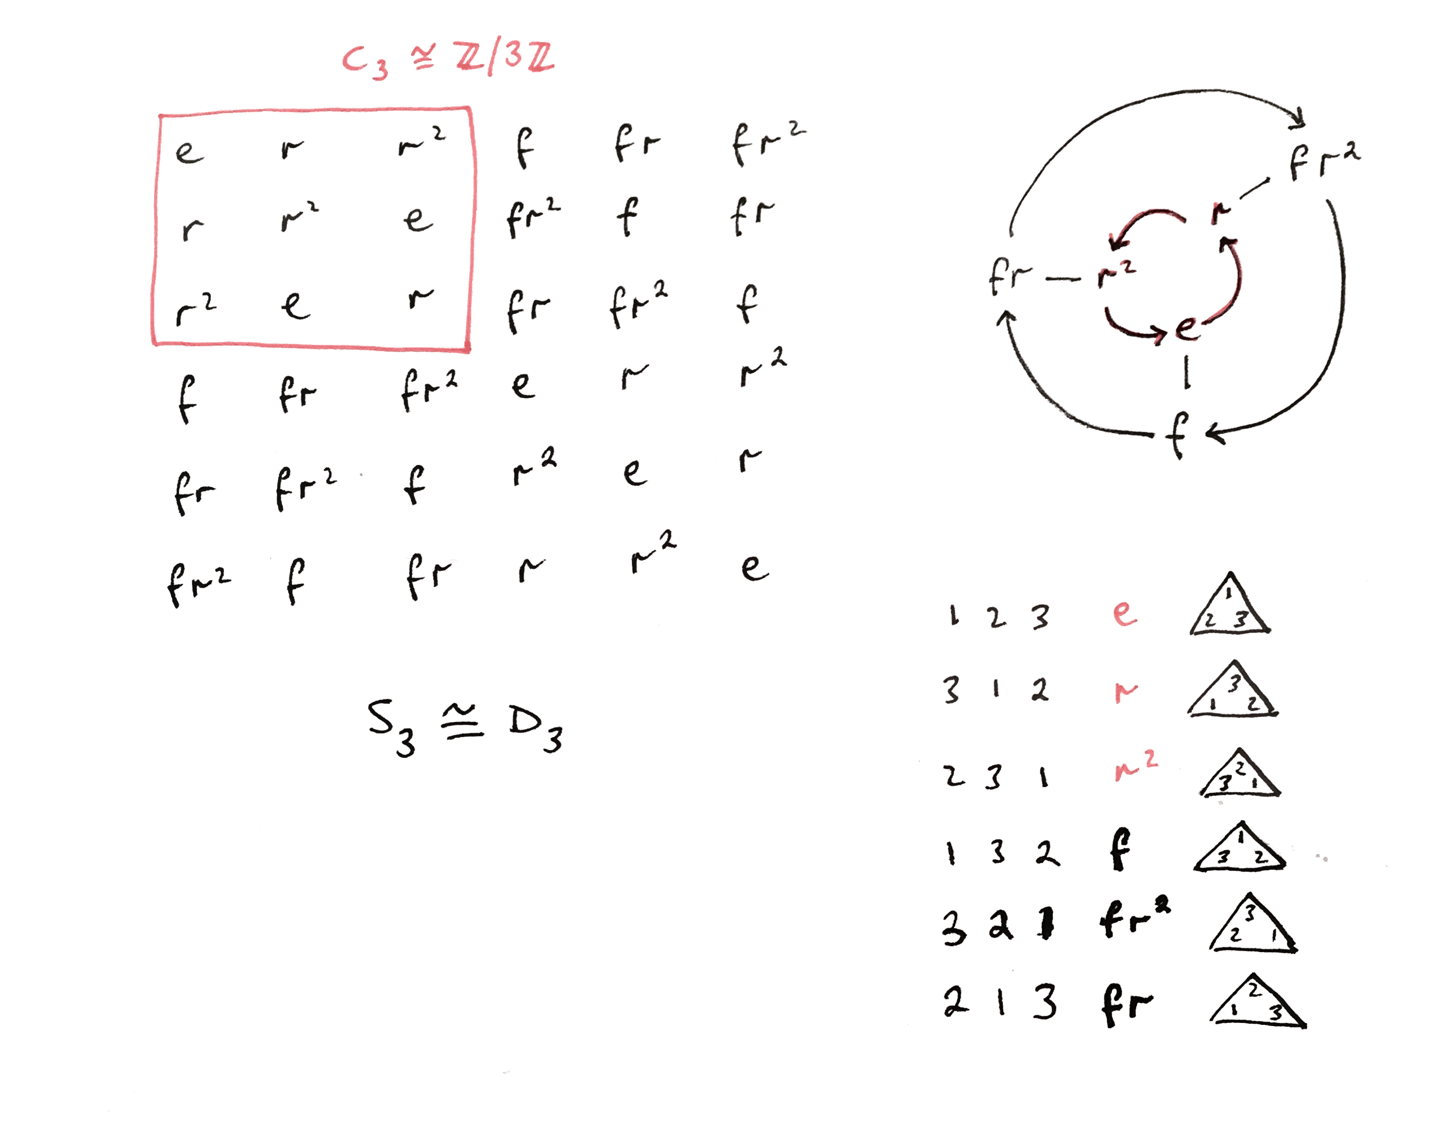
\includegraphics[width=400pt]{img/abstract-algebra-s3-d3.png}
  \end{mdframed}
\item $\{1, i, -1, -i\}$ where the operation is multiplication of complex numbers.
\end{itemize}

\subsection{Infinite order}

\begin{itemize}
\item The group $\Z$, i.e. integers under addition
  \begin{itemize}
  \item[$\diamond$] A homomorphism is $f:\Z \to \{0, 1\}$, given by $f(n) =
    \begin{cases}
      0, ~~\text{$n$ is even}\\
      1, ~~\text{$n$ is odd}\\
    \end{cases},$ with the operation on $\{0, 1\}$ being addition mod 2. The kernel is
    $evens = 2\Z$, and the resulting quotient group is
    $\Z/2\Z = \{evens, odds\} = \{2\Z, 2\Z + 1\}$.
  \end{itemize}

\item The ring $\Z$ - example of homomorphism.
\item $\Z_{>0}^+$ positive integers under addition

\item Similarly, $\Q^+$, $\Q^\times$, $\C^+$, $\C^x$, $\R^+$, $\R^x$ etc

\item $GL_n(\F)$: the set of $n \times n$ matrices with entries from the field $\F$, under matrix
  multiplication.
  \begin{itemize}
  \item[$\diamond$] A homomorphism is $f:GL_n(\F) \to \F^\times$ given by $A \mapsto \det(A)$. This
    is a homomorphism since $\det(AB) = \det(A) \det(B)$. The kernel is the set $SL_n(\F)$ of
    matrices with determinant 1. If the field is $\R$ then these rotate or flip space without
    stretching it. The resulting quotient group is the set $\{\mathcal{A}(x) ~|~ x \in \F\}$, where
    $\mathcal{A}(x)$ is the set of matrices with determinant $x$.
  \end{itemize}

\item The set $\F[x]$ of polynomials with coefficients in a field $\F$ can be a vector space, and a
  ring. (Not a field, since multiplicative inverses don't exist for degree $\geq 1$.)

  As a vector space, differentiation is a linear transformation (homomorphism). This is
  non-injective (polynomials differing only by an additive constant additive are sent to the same
  polynomial). The kernel is the set of degree 0 polynomials ($\F$). The quotient space $\F[x]/\F$
  contains cosets of the form $p(x) + \F$, i.e. a set of polynomials differing only by an additive
  constant.

  But differentiation does not preserve multiplication of polynomials, so it is not a ring
  homomorphism.

\item $SL_n(\R)$: set of $n \times n$ matrices with determinant $1$ (kernel of the
  determinant homomorphism $GL_n(\R) \rightarrow \R^\times$ and therefore a normal
  subgroup of $GL_n(\R)$)
\end{itemize}


\newpage
\section{Homomorphism}

A \textbf{homomorphism} is a map from one group to another. If it is bijective,
it is an \textbf{isomorphism}. If it is bijective and from a group to itself
(i.e. a permutation of the group elements) then it is an
\textbf{automorphism}. The critical feature of these concepts is that they
``preserve group structure'', i.e. they preserve the relationships among group
elements defined by the group operation. Suppose that they map from group $G$
to group $G'$. Then the preservation-of-structure criterion is that the map
sends a product $g_1 \circ g_2$ to the product of whatever the separate
elements are sent to:

$$
f(g_1 \circ g_2) = f(g_1) \circ f(g_2)
$$

There the composition on the left is happening in $G$ and the composition on
the right is happening in $G'$. (For an automorphism, $G=G'$.)

Another way of saying this is that ``the following diagram commutes'':
\begin{align*}
  \matMMMxNNN
  {g_1, g_2}{\xrightarrow{~~f~~}}{f(g_1), f(g_2)}
  {\Big\downarrow}{}{\Big\downarrow}
  {g_1g_2}{\xrightarrow{~~f~~}}{f(g_1g_2) = f(g_1)f(g_2)},
\end{align*}
i.e. it does not matter whether you first perform the internal structure operation on the left-hand
side and then apply $f$, or alternatively apply $f$ first and perform the internal structure
operation on the right-hand side.

Note that an element such as $g_1$ that is being sent somewhere by a morphism
may itself already be a map of sorts, e.g. if it is a permutation in
$S_3$. This is potentially confusing, since an automorphism can be thought of
as a permutation of group elements. So an automorphism on $S_3$ is a
permutation of group elements that are themselves permutations of some generic
labeled objects.

The definition of homomorphism implies that $f(g^{-1}) = f(g)^{-1}$ since
$f(gg^{-1}) = f(g)f(g^{-1}) = f(e)$.

\section{Kernel, Nullspace, Bijection and Congruency}

Consider a homomorphism $f$ with kernel $N$.

\textbf{Theorem:} $a$ and $b$ are sent to the same place by $f$ if and only if
$b = an$ for some $n \in N$.

\textbf{Corollary:} $f$ is a bijection (isomorphism) if and only if the kernel
contains only the identity element.

\textbf{Example:} Consider the absolute value homomorphism mapping complex numbers
under multiplication to positive reals under multiplication. The equivalence
classes are concentric circles around the origin. Two complex numbers have the
same absolute value iff one can be obtained from the other by rotation only (no
scaling). This is multiplication by a complex number with absolute value 1, and
such a complex number is in the kernel.

\textbf{Proof:} Clearly, if $b = an$ then $b$ is sent to the same place as $a$,
since

$$
f(b) = f(an) = f(a)f(n) = f(a).
$$

However we need to demonstrate the converse, i.e. that the *only* way that $b$
can be sent to the same place as $a$ is if $b=an$ for some $n \in N$.

Two almost identical ways of showing that:

\textbf{(1) Show that if $f(a) = f(b)$ then $b = an$ for some $n \in N$}

In linear algebra, you can always get from $u$ to $v$ by adding $v - u = -u +
v$, so the claim is that $L(u) = L(v)$ implies $-u + v$ is in the nullspace,
which is true:

$$
L(-u + v) = L(-u) + L(v) = L(-u) + L(u) = 0.
$$

For a group homomorphism, $b$ can be written as $aa^{-1}b$, so the claim is
that $f(a) = f(b)$ implies $a^{-1}b \in N$, which is true:

$$
f(a^{-1}b) = f(a^{-1})f(b) = f(a)^{-1}f(a) = e.
$$

\textbf{(2) Show that if it is not the case that $b = an$ for some $n \in N$, then $f(a) \neq f(b)$}

In linear algebra, you can always get from $u$ to $v$ by adding $v - u = -u + v$,
so if $-u + v$ is not in the nullspace then

$$
L(v) = L(u + (-u + v)) = L(u) + L(-u + v) \neq L(u).
$$

For a group homomorphism, $b$ can be written as $aa^{-1}b$, so if $a^{-1}b$ is
not in the kernel then

$$
f(b) = f(aa^{-1}b) = f(a)f(a^{-1}b) \neq f(a)
$$


\section{Inverse of an automorphism is an automorphism}

[Artin 2.3.11: show that Aut($G$) is a group]

Suppose $\alpha$ is an automorphism that sends $g_1$ and $g_2$ to $g_1'$ and
$g_2'$, respectively.

\begin{mdframed}
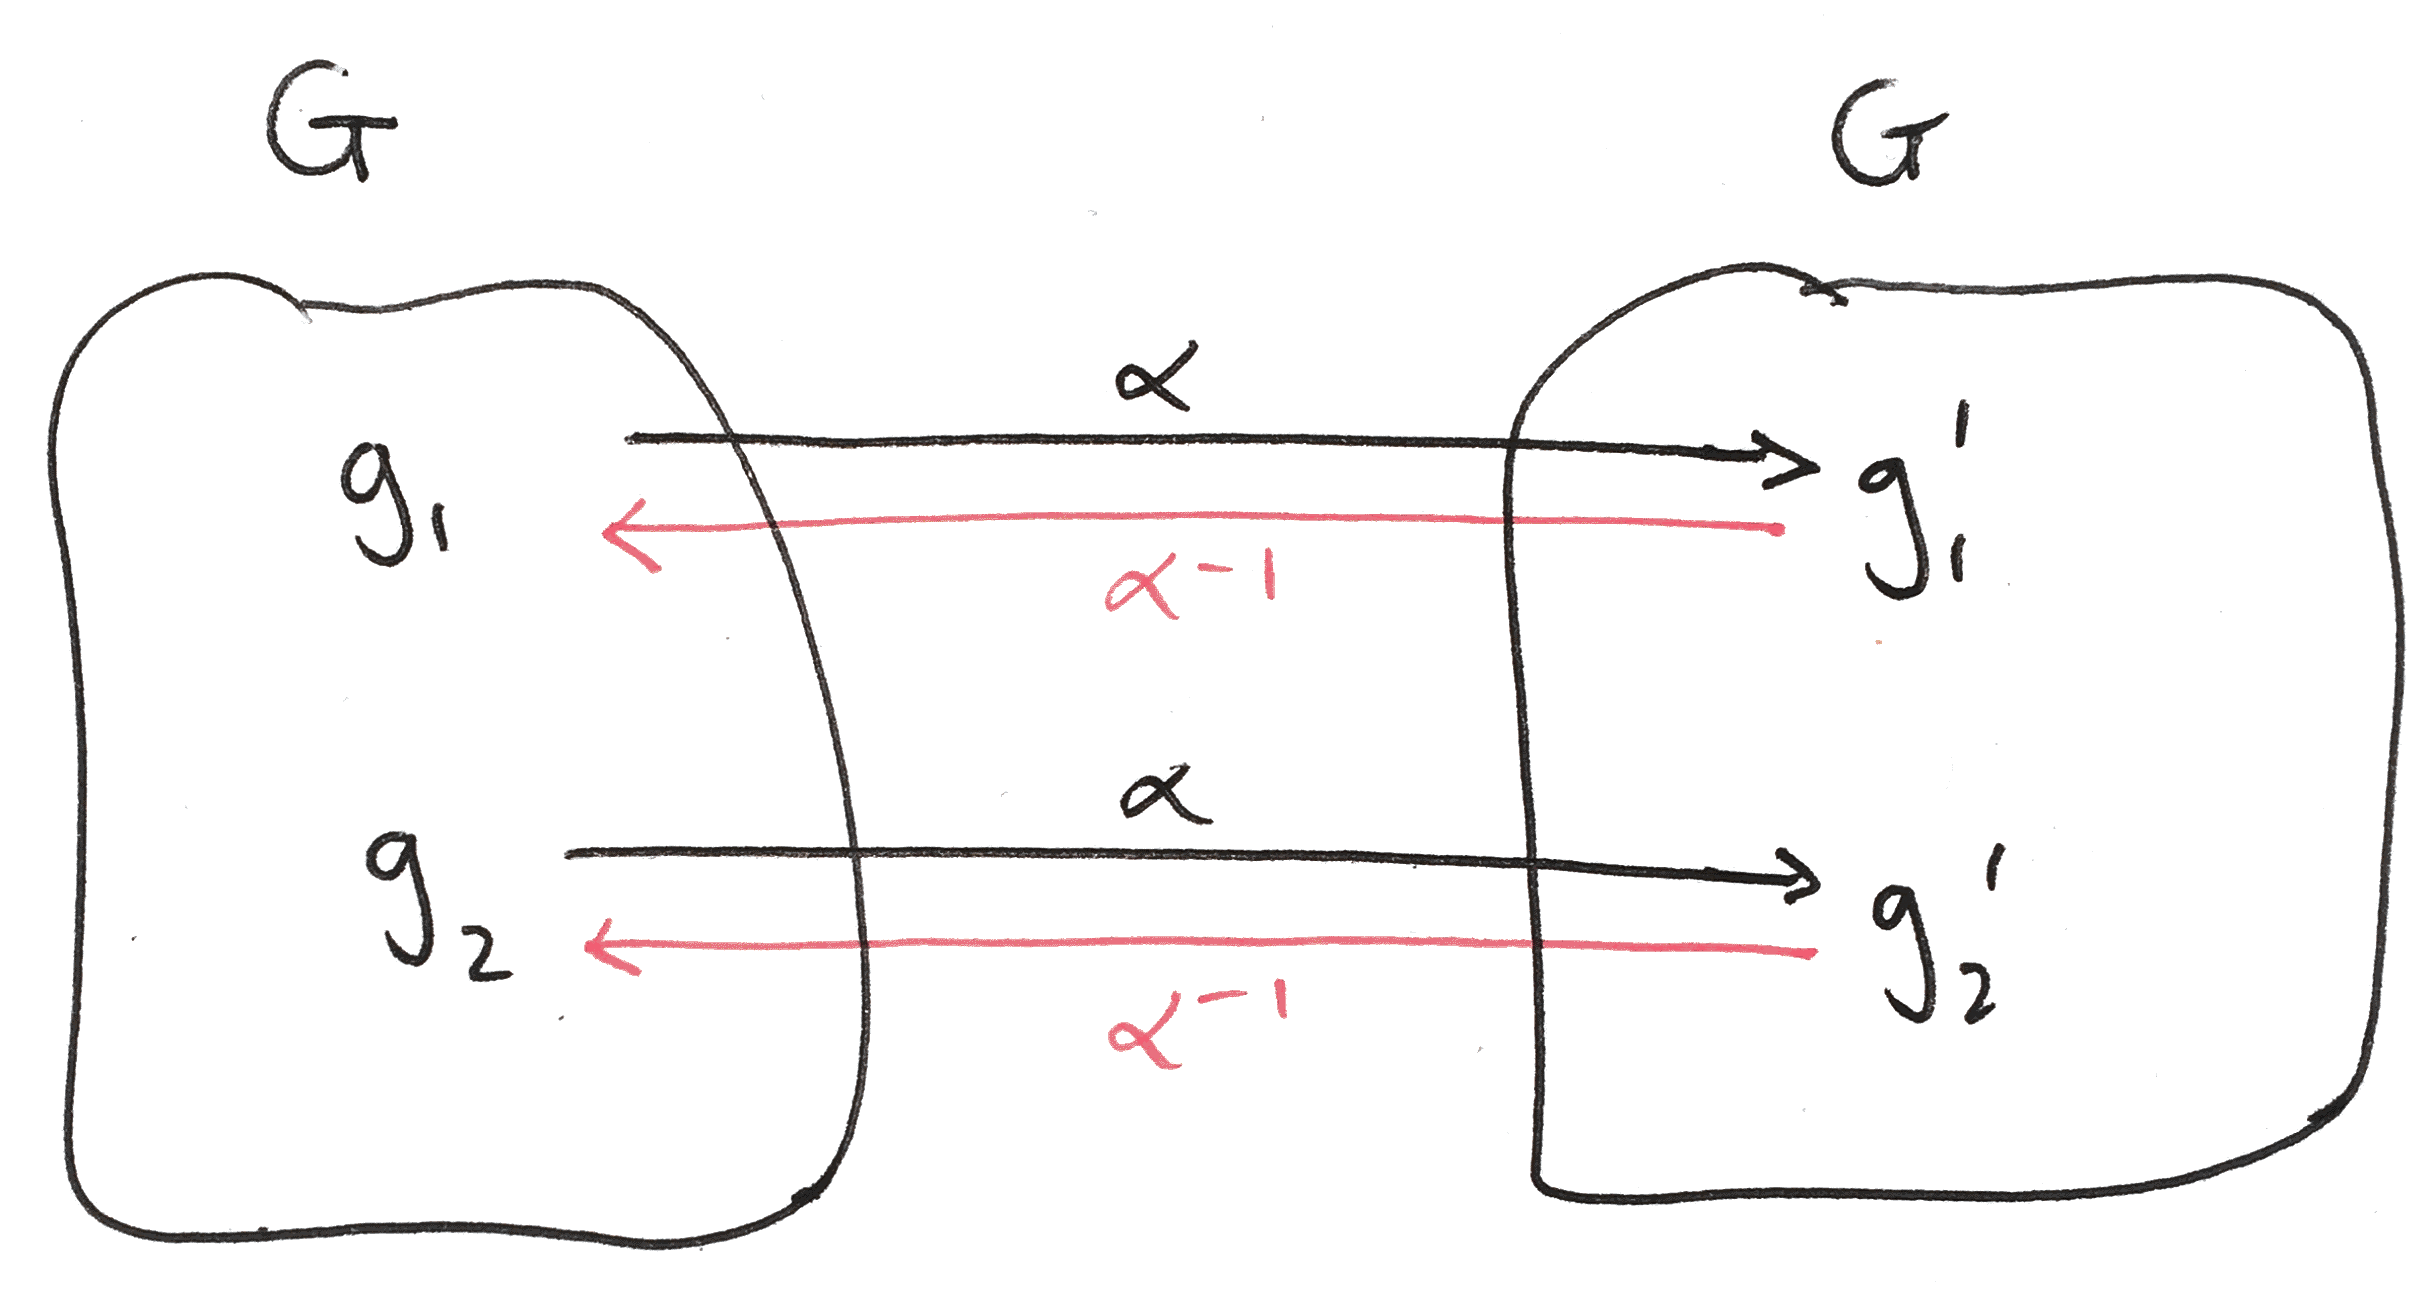
\includegraphics[width=300pt]{img/inverse-of-automorphism-1.png}
\end{mdframed}

We need to show that $\alphainv$ preserves structure, i.e. that when $\alphainv$ acts
on an element which is a product, say $g_1'g_2'$, it sends it to the product of
whatever it send the individual factors to:

$$
\alphainv(g_1'g_2') = \alphainv(g_1')\alphainv(g_2').
$$


Firstly, we know that $\alphainv(g_1')$ and $\alphainv(g_2')$ exist, i.e. some elements
are taken to them by $a$, because $a$ is an automorphism and therefore
surjective. So we'll call those $g_1$ and $g_2$, and the equality we need to
demonstrate has become

$$
\alphainv(\alpha(g_1)\alpha(g_2)) = g_1g_2.
$$

Since $\alpha$ is an automorphism, it preserves structure, therefore
$\alpha(g_1)\alpha(g_2) = \alpha(g_1g_2)$. So,

$$
\alphainv(\alpha(g_1)\alpha(g_2)) = \alphainv(\alpha(g_1g_2)) = g_1g_2,
$$

as required.
\newcommand{\textstack}[2]{
  \left(\begin{array}{c}
    \text{#1}  \\
    \text{#2}
  \end{array}\right)
}

\section{Quotient groups}

\subsection{Quotient groups and the first isomorphism theorem in plain English}
\begin{enumerate}
\item You have groups $G$ and $H$ and a homomorphism $f:G \to H$. That is special; it is not just
  any map.
\item You use the values of $f$ to define an equivalence relation $\sim$ on $G$. That's not
  special, you could do that with any map.
\item Note that this will only be interesting if $f$ is non-injective, i.e. if the equivalence
  relation does actually group some elements together.
\item You define a group operation on the equivalence classes of $G$. This is ``inherited from the
  underlying group''\footnote{ What this means is that the rule for combining equivalence classes
    is as follows:
  \begin{enumerate}
  \item Pick an arbitrary element of each equivalence class.
  \item Combine those two elements according to the group operation.
  \item Declare the result of the operation on equivalence classes to be the equivalence class of
    the group-element level result.
  \end{enumerate}
}.

So far everything has been straightforward; here is the only subtle point:

It is essential that the operation defined on the equivalence classes is well-defined. Fortunately,
it will be. Ultimately, the reason is that the equivalence classes were defined by the values of a
homomorphism, not just any arbitrary labeling.
\item So now you have a new group $G/{\sim}$ containing equivalence classes. There are four
  interesting things about it:
  \begin{enumerate}
  \item Obvious: It is smaller (simpler) than the original group $G$: you have ``modded out'' by
    the equivalence relation.
  \item Somewhat obvious: All information about the original group structure on $G$ is preserved in
    the group structure on $G/{\sim}$. This is because we decided that the group operation on the
    equivalence classes would be inherited from $G$.
  \item Obvious: There is a one-to-one correspondence between the equivalence classes and the image
    of the homomorphism (the elements of the image ``label'' the equivalence classes).
  \item Somewhat obvious: this one-to-one correspondence is actually an isomorphism.

    Why? We started off with a non-injective homomorphism $G \to H$. Then we did two things: (1) we
    coalesced into a single new element all the elements in $G$ that mapped to the same element in
    $H$; (2) we declared that the new coalesced element on the left
  \end{enumerate}
\end{enumerate}

\newpage
\begin{theorem}[First Isomorphism theorem: statement I]~\\
  Let $f:G \to H$ be a group homomorphism.

  Let $\sim$ be the equivalence relation on $G$ defined by $g_1 \sim g_2 \iff f(g_1) = f(g_2)$.

  Then the set $G/{\sim}$ of equivalence classes ``inherits the structure'' of $G$ in the following
  sense:

  Let $C_1, C_2 \in G/{\sim}$ be equivalence classes with $g_1 \in C_1$ and $g_2 \in C_2$. Define
  $C_1C_2 := $ (equivalence class of $g_1g_2$). Then this is well-defined and $G/{\sim}$ is a group
  under this operation.

  \red{TODO: state something about isomorphism of $G/{\sim}$ and $\Im f$. The group operation in
    $H$ could be anything; all we know is that $f:G \to H$ is a homomorphism. And the group
    operation in $G/{\sim}$ is inherited from $G$. The point here is that the map
    $G/{\sim} \to \Im f$ is a homomorphism, just as the original map $f:G\to H$ was. In fact, it's
    an isomorphism, because it is a bijection.}
\end{theorem}

\begin{remark*}~\\
  Note that the equivalence class of $g_1$, i.e. the preimage of $f(g_1)$, is
  \begin{align*}
    f^\1(f(g_1)) = g_1\cdot\Ker f.
  \end{align*}
  This is true since, (reverse direction) if $k \in \Ker f$, then $f(g_1k) = f(g_1)e = f(g_1)$; and
  (forwards direction) if $f(g_2) = f(g_1)$ then (\red{TODO: prove subset in this direction}).

  Therefore an equivalent definition of the equivalence relation is:

  $G/{\Ker f} := G/{\sim}$, where $g_1 \sim g_2 \iff (g_1\cdot \Ker f) = (g_2\cdot \Ker f)$.

  $G/{\Ker f}$ is a set of cosets of $\Ker f$, and may also be thought of as a set of equivalence
  classes of $\sim$.

  This gives rise to the conventional statement of the theorem:
\end{remark*}

\begin{theorem}[First Isomorphism theorem: statement II]~\\
  Let $f:G \to H$ be a group homomorphism.

  Then the set $G/{\Ker f}$ ``inherits the structure'' of $G$ in the following sense:

  Let $C_1, C_2 \in G/{\Ker f}$ be cosets of $\Ker f$, with $g_1 \in C_1$ and $g_2 \in C_2$. Define
  $C_1C_2 := $ ($g_1g_2\cdot \Ker f$). Then this is well-defined and $G/{\Ker f}$ is a group under
  this operation.

  \red{TODO: state something about isomorphism of $G/{\Ker f}$ and $\Im f$.}
\end{theorem}




\subsection{Summary}
A quotient group can be formed by:
\begin{enumerate}
\item Identify a subgroup
\item Form cosets
\item Inherit operation on cosets from operation on original group elements
\end{enumerate}
But only if the subgroup is normal: that's what's required for inheriting the group operation to
result in a well-defined operation on the cosets (i.e. when performing an operation involving
members of two different cosets, all choices of members to act as exemplars of the cosets give the
same result.)

\subsection{Modular arithmetic}

The canonical example of a quotient group comes from "modular arithmetic" on
the integers. For example, consider the integers, mod 4. This means that every
integer is mapped to whatever its remainder is after dividing by 4. The
integers mod 4 is a group, which contains 4 elements: $\{\bar 0, \bar 1, \bar
2, \bar 3\}$. So $5 \rightarrow \bar 1$, $14 \rightarrow \bar 2$, $-1
\rightarrow \bar 3$, etc.

We said that the integers mod 4 are a group, so what is the group operation?
The answer is that we define an addition law on the elements: for example,
$\bar 1 + \bar 3 = \bar{1 + 3} = \bar 4 = \bar 0$. In words, to find the result
of combining $\bar 1$ with $\bar 3$, you first add $1$ and $3$ as usual to get
4, then see where $4$ is mapped to, and that's the answer. This corresponds to
the fairly familiar notion that e.g. $5 + 23 = 28 = 0$ (mod 4), but it is a bit
subtle/slippery, and it helps to pause and consider exactly what's going on.

Let's be explicit about what $\bar 1$ actually is: it's the set of all integers
that have $1$ as their remainder when divided by $4$. So, $5 \in \bar 1$ for
example. What we've just done is define an addition operation on these
\emph{sets} (as opposed to addition of integers). The operation works as
follows. To add $\bar 2$ and $\bar 3$, you do the following:

1. Take any number that has remainder $2$ (mod $4$) and any number that has
   remainder $3$ (mod $4$).
2. Add them together using normal integer addition and find the remainder (mod
   $4$) of the result.

There are two important points here.

Firstly, we didn't need anything beyond what we had to come up with this
operation: it uses the addition operation that's \emph{already defined} on the
main group to define an operation on the subsets.

Secondly, it is only well-defined if you always get the same answer regardless
of which integers you pick in step (1). In this case that is true.

So we have an example of a ``quotient group'': $\{\bar 0, \bar 1, \bar 2, \bar
3\}$ under this addition operation. Let's recap and start putting this in group
theoretic terminology.

\footnotetext{Multiplication preserves structure also: $\Z/n\Z$ is a field iff
  $n$ is prime.}

\subsection{A quotient group is a group of cosets}

$\bar 0$ (mod $4$) is the following subset of the integers $\Z$ under addition:
$\{\ldots, -12, -8, -4, 0, 4, 8, 12, \ldots\}$. It's not only a subset, but a
\emph{subgroup} (it contains the identity element $0$, every element has an
additive inverse, and addition stays within the subset). It is written as $4\Z$
(or in general, $n\Z$ for mod $n$). However, we will often use $H$ for a
subgroup, so let's call it $H$.

$\bar 1 = \{\ldots, -11, -7, -3, 1, 5, 9, 13, \ldots\}$ is not a subgroup of
$\Z$ because it does not contain the identity element. What it is is a
\emph{coset} of the subgroup $H$: the set comprising all the results you get by
adding $1$ to elements of $H$. We can write this as $1 + H$. In fact, it's
usually written $1H$; we just have to remember that the operation here is
additive rather than multiplicative.

Of course, $\bar 2$ and $\bar 3$ are cosets defined in the same way. $\{\bar 0,
\bar 1, \bar 2, \bar 3\}$ are the only distinct cosets: for example, $\bar 4 =
4+H$ is exactly the same set of integers as $\bar 0$. Similarly, $5 + H = \bar
1$, etc.

So we arrived at the (integers mod $4$) quotient group as follows:

\begin{enumerate}
\item We started with the group of integers under addition, $\Z^+$.
\item We identified a subgroup $H$.
\item We identified the cosets of $H$: $\{H, 1+H, 2+H, 3+H\}$
\item We defined an operation on the cosets: $(i+H) + (j+H) = (i+j)+H$.
\item We noted that it was only well-defined because
  \begin{align*}
    \textstack{any number with}{remainder $i$} +
    \textstack{any number with}{remainder $j$} =
    \textstack{a number with the same}{remainder as $i+j$}.
  \end{align*}
\end{enumerate}

Note that (3) and (4) can equally be written like this, which is how it's
likely to be written when considering subgroups and cosets more abstractly:

\begin{enumerate}
\item We identified the cosets of $H$: $\{H, 1H, 2H, 3H\}$
\item We defined an operation on the cosets: $(iH) + (jH) = (ij)H$.
\end{enumerate}

\subsection{Notational digression}

The integers mod $4$ is written $\Z/4\Z$. It's an example of a quotient
group. You read that as $(\text{some group}) / (\text{some subgroup})$. In this
case the group is the integers under addition, and the subgroup is
$4Z = \{\ldots, -12, -8, -4, 0, 4, 8, 12, \ldots\}$\footnote{In this context,
  $4\Z$ always means multiplication, even if the group operation is addition!
  So it's the set $\{4z|z \in \Z\}$. It is \emph{not} the same as the coset
  $4 + \Z = \{4+z|z \in \Z\}$. This is a well-established notational
  inconsistency.}. In general, one writes $G/H$ to refer to the quotient group
of "$G$ mod $H$".


\subsection{A second example of a quotient group}

Here's an example of a (simple) problem from an undergraduate textbook on group theory:\\

\begin{mdframed}
  Identify the quotient group $\R^\times/P$, where $P$ denotes the subgroup of
  positive real numbers.
\end{mdframed}

What does this mean and how does one do it? Well, let's try to follow the same
steps as for the integers mod $4$ example above.

Our starting group is the non-zero real numbers under multiplication $\Rx$:
this plays the role of $\Z^+$ in the modular arithmetic example. And the
subgroup is the positive real numbers $P$.

What are the cosets of $P$? To get one example of a coset, you pick a number
$x$ from the main group, and you form a set by combining $x$ with each element
of the subgroup $P$ in turn. So that's the set $\{xp|p \in P\}$. We can see
that we're either going to get all the positive reals (if $x$ is positive), or
all the negative reals (if $x$ is negative). So the set of cosets has those two
sets as its elements: $\{P, -1P\}$.

OK, so we've done steps (1)-(3). Now, what's the group operation that's going
to combine two cosets and produce another coset? Well, the whole point is that
this group operation is inherited from the original group: that's what we did
in the integers mod $4$ example; we used the standard addition of integers to
define the result of adding cosets $i+H$ and $j+H$ to be the coset
$(i+j)+H$. The analogous definition here would be to use the standard
multiplication of real numbers to say that $(xP)(yP) = (xy)P$. That's going to
lead us to the following intuitively reasonable multiplication table:

$$
\begin{array}{ c|cc }
 ~   & P   & -1P \\
 \hline
 P   & P   & -1P \\
 -1P & -1P & P \\
\end{array}
$$

And we conclude that the quotient group is isomorphic to the group of size 2
(there's only one -- the one with this multiplication table).

The only question is (5): is the operation on cosets well-defined? In this
case, the answer is yes: for example, any positive number $x \in P$, multiplied
by any negative number $y \in -1P$, is going to give a negative number $xy \in
-1P$.\footnote{We can prove it easily here because the group is commutative:
$(xP)(yP) = (Px)(yP) = P(xy)P = (xy)PP = (xy)P$. In addition to commutativity
those steps make use of associativity and closure.}.


\subsection{Quotient groups of arbitrary groups}

What about in general? If we have a subgroup, can we just identify the cosets
of the subgroup, and define a composition law on them using the composition law
from the main group? Will it always be well-defined in the sense answered
above? The answer is: yes if and only if the subgroup is ``normal''.

A normal subgroup $H$ is defined to be a subgroup that is closed under
conjugation. This means that you can take any element $g$ of the main group,
form the product $ghg^\1$ using any element $h$ of the subgroup, and the result
will always be in the subgroup. One can prove that if and only if this is true,
then the composition of cosets is well-defined, in which case the prescription
above for forming a quotient group can be followed (find the cosets of $H$,
define the operation on the cosets).

So, if you need to find a quotient group of some subgroup, you need to show
that the subgroup is normal. There are two ways of doing that:

\begin{enumerate}
\item Show that it is closed under conjugation.
\item Show that it is the kernel of a homomorphism.
\end{enumerate}

\newpage
\subsection{Quotient groups}
\footnotetext{Notes based on Tim Gowers' blog \url{https://gowers.wordpress.com/2011/11/20/normal-subgroups-and-quotient-groups/}}

A mapping $f$ \underline{preserves structure} if, for example:
\begin{align*}
  a  & \mapsto f(a)\\
  b  & \mapsto f(b)\\
  ab & \mapsto f(a)f(b)
\end{align*}

An \underline{isomorphism} is a bijection that preserves structure.

A \underline{homomorphism} is a mapping that preserves structure but isn't
necessarily a bijection.\footnote{I.e. it might not be injective (might send
  different inputs to the same output), or might not be surjective (might fail
  to hit certain elements).}

\begin{theorem}
The \underline{kernel} of a homomorphism is a \underline{subgroup} \footnote{\textbf{Proof.}\\Kernel
  is $\{a:f(a) = e\}$.\\
Contains identity? Yes, homomorphisms always send the identity to the identity
($f(ea) = f(e)f(a)$ but this must equal $f(a)$, hence $f(e)$ is the identity.)
Contains inverses? Yes, $f(aa^\1) = f(a)f(a^\1) = ef(a^\1) = e$, so $f(a^\1)$ must also be $e$.}.
\end{theorem}

\textbf{Example}: the group of \emph{rotations} of $\R^3$ is a subgroup of the
group of rigid motions that fix the origin (the latter includes
reflections). Now the $\det:\GLR{3} \to \R$ mapping is a homomorphism, since
$\det(T_1T_2) \equiv \det(T1)\det(T_2)$. The rotations are those mappings with
determinant 1, hence they are the kernel of a homomorphism.

\begin{theorem}
Some subgroups are not the kernel of any homomorphism
\end{theorem}

The counter example given in the proof (below) is an element of the form
$g^\1hg$ for $h$ in the subgroup and $g$ outside the subgroup. Basically, we
observe that
\begin{align*}
\varphi(g^\1hg) =
\varphi(g^\1)\cdot\varphi(h)\cdot \varphi(g) =
\varphi(g^\1)\cdot e\cdot\varphi(g) =
\varphi(g^\1)\cdot \varphi(g) =
\varphi(e) =
e,
\end{align*}
and therefore that the subgroup, if it is to be a kernel, must \emph{contain}
all products of the form $g^\1hg$ (conjugation by an element outside the
subgroup).

So,
\begin{align*}
  \textbf{kernel of homomorphism} \implies \textbf{closed under conjugation}.
\end{align*}
But does
\begin{align*}
  \textbf{closed under conjugation} \implies \textbf{kernel of homomorphism} ~ ?
\end{align*}
Yes. Closure under conjugation implies that the \textbf{subgroup is the kernel
  of the homomorphism which maps $g$ to its coset, with the operation on cosets
  inherited from the group}: $(g_1H) \cdot (g_2H) = g_1g_2H$. Justification of
this claim follows.

Suppose that $\varphi:G \to K$ is a homomorphism from $G$ to some group $K$,
and that the kernel of $\varphi$ is $H$ and that $H$ is closed under
conjugation. What can we deduce about $\varphi$?

\begin{theorem}~\\
  The left and right cosets of $H$ coincide, and $\varphi$ is constant on
  the cosets, taking different values on each coset.
\end{theorem}

This means that there is a \underline{bijection} between the cosets of $H$ and
the \underline{image} of $\varphi$. So, we can say that the image of $\varphi$
\textit{is} the cosets of $H$.

\begin{theorem}~\\
  If $\varphi(g_1H) = a_1$ and $\varphi(g_2H) = a_2$ then
  $\varphi(g_1g_2H) = a_1a_2$.
\end{theorem}

This allows us to define the group operation on the elements of the image of
$\varphi$: it implies that
\begin{align*}
  (g_1H) \cdot (g_2H) = g_1g_2H.
\end{align*}

\begin{theorem}
\begin{align*}
  \textbf{kernel of homomorphism} \iff \textbf{closed under conjugation} \iff gH = Hg ~~~ \forall g \in G
\end{align*}
\end{theorem}

~\\~\\~\\~\\~\\
\hrule
\begin{theorem*}
  Some subgroups are not the kernel of any homomorphism.
\end{theorem*}

\begin{proof} \label{some-subgroups-not-kernel}
Counter-example: consider the permutation group
$S_3 = \{e, (12), (13), (23), (231), (312)\}$, and its subgroup $\{e,
(12)\}$.

Suppose this subgroup is the kernel of a homomorphism. I.e.
$e \mapsto e, (12) \mapsto e$, but nothing else is sent to the identity.

Now consider $(13)(12)(13)$:
\begin{align*}
  123 \to 321 \to 231 \to 132,
\end{align*}
i.e. $(13)(12)(13) = (23)$.

But
\begin{align*}
  \varphi\Big((13)(12)(13)\Big) =
  \varphi\Big((13)\Big) \varphi\Big((12)\Big) \varphi\Big((13)\Big) =
  \varphi\Big((13)\Big) \varphi\Big((13)\Big) = \varphi\Big((13)(13)\Big) = e,
\end{align*}
so $(23) \mapsto e$, which is a contradiction. Therefore $\{e,(12)\}$ isn't the
kernel of any homomorphism.
\end{proof}

\begin{theorem*}
  The left and right cosets of $H$ coincide, and $\varphi$ is constant on the
  cosets, taking different values on each coset.
\end{theorem*}

\begin{proof}
  TODO
\end{proof}


\begin{theorem*}~\\
  If $\varphi(g_1H) = a_1$ and $\varphi(g_2H) = a_2$ then
  $\varphi(g_1g_2H) = a_1a_2$.
\end{theorem*}

\begin{proof}
  TODO
\end{proof}
\newpage
\subsection{First isomorphism theorem}

\footnotetext{\url{https://theoremoftheweek.wordpress.com/2010/05/20/theorem-26-the-first-isomorphism-theorem/}}

Every normal subgroup is the kernel of the homomorphism that sends a group element to its coset.

Can two distinct homomorphisms share the same kernel?

Let $f: G \rightarrow G'$ be a homomorphism with kernel $N$. $e \in N$,
therefore every $g \in G$ is in some coset $gN$, so the set of cosets
partitions the domain. What about the image? Consider two elements $gn_1$ and
$gn_2$ of the same coset. These both get sent to the same value, since
$f(gn_i) = f(g)f(n_i) = f(g)$.

So is it possible to have homomorphisms $f$ and $\varphi$ with the same kernel
$N$ but with $f(g) \neq \varphi(g)$ for some $g \in G$? If that were true [...]
